\section{Witnesses}
\frenchspacing

Hanneder's Intro to Text Genealogy, Textual Criticism 
and Editorial Technique(Introduction): very useful summary, use it!
\mycite{HannederIntro}
p. 5: `textual criticism is often viewed as something to be learned by practice rather from reading about it.'
ibid.: `In fact, both translating and editing are something most Indologists have learned in a pragmatic
way through examples from within the field, and some have managed to become quite good at it.'
ibid.: `in most cases this approach is sufficient'

p.7: basic method is common errors; age of mss, and number of mss preserving a reading is insignificant; Maas: only works if no contamination [but VSS must be deeply contaminated]

p. 11: Lachmann's objective method with no subjective judgement (recensio sine interpretatione) 
ibid.: `It seems that from these principles only the preference for the \textit{lectio difficilior} 
made it into text-critical modernity, and
even there reliance on it is sometimes rejected as too dangerous.' Also uncommon and offensive readings are preferred. But nothing can be followed mechanically. inner criteria

clearly not one author here; revisions?
Reject phyogenetics slightly
Even the best mss can containing a bewildering number of problematic readings, and
`worse' mss can give us clues as to how to emend the text...
Mention MaSa.m: there was a stemma, but it was useless
music: practice and theory
It is a skill.
Mention Sanderson's approach. 

\noindent
In the pre-modern era, the \VSS\ has been transmitted exclusively in multiple-text manuscripts that were produced in Nepal. Even when a
manuscript of the \VSS\ seems to be a single-text MS, 
chances are high that it originally belonged to a multiple-text
manuscript.%
	\footnote{\label{noteonKolkataMs}As I remarked elsewhere 
	(\mycitep{KissVolume2021}{185, n.~9}):
	`Asiatic Society (Calcutta), Manuscript G 4076, cat. no. 4083, 
	may seem to be an independent manuscript of the 
	\textit{Vṛṣasārasaṃgraha}, but as De Simini has already 
	remarked (2016b, 240 n. 19) [= \mycite{DeSiminiMSSFromNepal2016}],
	it is probably from a multiple text manuscript. In fact, from what
	can be gathered from its description in
	\mycitep{shastri_descriptive_1928}{716ff},
	it seems likely that this manuscript was
	originally part of manuscript Asiatic Society (Calcutta) G 3852, cat.\
	no.\ 4085. See for example the folio numbering in these two 
	manuscripts: ASC G 3852 contains 210 folios, 
	and ASC G 4076 starts on folio 210.'}
In the manuscript descriptions below, in addition to some general
remarks, I will mainly focus on information relevant to the \VSS. For
much more detail on the overall features of these manuscripts, see 
\mycite{DeSiminiMSSFromNepal2016} and the catalogues I mention
at some of the individual manuscript.%
		\footnote{I owe thanks to Florinda De Simini for 
			sharing with me most of the manuscripts listed here, to
  			Kengo Harimoto and Gudrun Melzer (Munich) for 
  			providing photos of the  Munich MS, and to 
  			Nirajan Kafle for sharing a digital 
  			copy of the Paris MS with me.}

In recently published and forthcoming critical editions of and articles
on the Śivadharma corpus 
(e.g. \mycite{BisschopUniversal2018} and 
\mycite{SaivaUtopia2021}), 
the sigla of the manuscripts used are made up of 
a letter signifying the script (e.g.~`N' for
Nepālākṣara/Newari), a superscript letter for the current location where
the manuscript is deposited (e.g.~`C' for Cambridge), and two (sometimes only one or even three) subscript digits echoing the last digit(s), if any, of the reference number of the manuscript in the 
library where it is located or, in the case of NGMPP reel 
numbers, the last two digits of the first part of the reel number. 
For details of this system and for the underlying reasons, see 
\mycitep{BisschopUniversal2018}{50--51}. 
Since in the case of the \VSS\ all available 
manuscripts use some variant of the Nepālākṣara script, 
in this publication I omit the first letter, making the letter for the current 
location non-superscript. This helps keeping the apparatus 
readable. In the manuscript descriptions below, I give this 
omitted and implied `N' in brackets as a reminder.

%\section{How to describe a MS?}\label{how-to-describe-a-ms}

%In general these categories should be included: - {[}X{]} Siglum - {[} {]} Location where it is deposited - {[} {]} Ms no. - {[} {]} How much do I use it? - {[} {]} Catalogued by and where and under what no., with what title - {[} {]} what does the catalogue says - {[} {]} Physical: - {[} {]} material - {[} {]} dimensions - {[} {]} no of folios - {[} {]} condition - {[} {]} format, binding - {[} {]} Text - {[} {]} script - {[} {]} contains these texts - {[} {]} complete - {[} {]} language (implied) - {[} {]} MTM? - {[} {]} foliation - {[} {]} hands - {[} {]} initial rubric, incipit, explicit, final rubric (in edition) - {[} {]} colophons (in edition) - {[} {]} dating - {[} {]} description in detail, remarks

\medskip
\subsection{The Cambridge manuscripts}

\mysubsubsection{(N)\msCa}{nc94}
Cambridge University Library, Add. 1694.1. This MS has been 
fully collated for chapters 1--12 of the critical edition in this volume. 
See a detailed description of this manuscript in the 
CUDL online catalogue.\footnote{https://cudl.lib.cam.ac.uk/view/MS-ADD-01694-00001/382}
According to this catalogue, the date of creation of this manuscript 
is the 12th century, its dimensions are 5 × ca.\thinspace 53.5 cm. 
The script is Nepālākṣara. It is a palm-leaf multiple-text manuscript containing 258
folios and transmitting eight texts: 
1)~\SDhS,
2)~\SDhU,
3)~\SDhSangr,
4)~\Ums,
5)~\Uums, 
6)~\Vss,
7)~\DharmP,
8)~\SivaUp.

The \VSS\ occupies 45 folios: it starts on \fol193 
(the recto side, online image no.\thinspace381, is an empty folio side,
the text itself starts on the verso side); 
it ends on \fol239r (online image no.\thinspace473). 
The text of the \VSS\ is transmitted fully,
without any folios or major sections of the text missing. The leaves
transmitting the \VSS\ are well-preserved. Some folio sides are faded and
most folios are somewhat damaged on the right side, sometimes at other parts, and it seems from the images that some opaque-looking tape has been applied to protect these damaged sections. 
In my critical edition
the broken off, completely lost, \emph{akṣara}s are represented by \lost,
the illegible \emph{akṣara}s under the tape by \il\ (`illegible'). The
quality of the readings of this manuscript is one of the best among
the available witnesses, comparable only to \msNa\ and \msP, 
making it one of the most important sources for the \VSS.


\mysubsubsection{(N)\msCb}{nc45}
Cambridge University Library, Add. 1645. This MS has been fully
collated for chapters 1--12 of the critical edition in this volume. 
See a detailed description of this manuscript in the CUDL online catalogue.\footnote{https://cudl.lib.cam.ac.uk/view/MS-ADD-01645/404}
According to this catalogue, the dimensions of the manuscript are 
4.4 × 61.7 cm. The manuscript is dated to (Nepala) `\emph{samvat} 259
\emph{śrāvaṇa śukla dvādaśiyādi}(?) \textless{} \emph{trayodaśyām},'
which converts to July 10/11 Monday/Tuesday, 1139 \CE.%
		 \footnote{\Fol247r line 6. The CUDL website transcribes this
		  colophon as: \emph{saṃvat} 259 
		  \emph{śrāvaṇaśukladvādaśi{\rm[}pyaḍi} 8 
		  \emph{trayodaśyāṃ} (retrived 8 Dec 2021). 
		  The element \emph{dvādaśipyaḍi} might be read as
		  \emph{dvādaśiyā} \emph{di}, perhaps a mistake for
		   \emph{dvādaśyāṃ}
		  \emph{di} (\emph{di} for a misplaced \emph{diva/divā}?), and the
		  symbol that does look like a figure `8' of a slightly later period
		  than the manuscript itself (resembling the mathematical symbol
		  \textless{}) might also be a \emph{kākapada}. Another faint
		  \emph{kākapada} is perhaps to be seen under \emph{daśi},
		  therefore it is possible that the scribe's intention was to delete 	
		  \emph{dvādaśi}° and correct it to \emph{trayodaśyām}, 
		  and then the date becomes 11th of July. Kengo Harimoto 
		  has suggested that the unclear element
		  (\emph{yādi/pyaḍi}) is in fact \emph{ghaṭi}, 
		  and after comparing these two syllables to other instances of
		   \emph{gha} and \emph{ṭa}, one cannot but agree. 
		   In this case this should be an indication of the
		  exact time (\skt{ghaṭikā}) 
		  the scribe finished copying the text. It is still not clear
		  if we should take \emph{dvādaśi} or \emph{trayodaśyām} 
		  as the date. For help on the conversion of the date and 
		  for a detailed discussion on the colophon I am indebted
		  to Kengo Harimoto.} 
The script is Nepālā\-kṣara. It is a palm-leaf multiple-text manuscript containing 247 folios. Eight texts are transmitted in this manuscript: 
1)~\SDhS,
2)~\SDhU,
3)~\SDhSangr,
4)~\SivaUp,
5)~\Ums,
6)~\Uums, 
7)~\Vss,
8)~\DharmP.


The VSS occupies 37 folios plus one folio side: it starts on \fol201v
line 4 (online image no.\thinspace 404), 
and it ends on \fol238v line 3 (online image
no.\thinspace 478). 
The readings of this manuscript seem to follow those of \msNa\
remarkably closely while transmitting the 
Śivadharmottara (as observed by De Simini and Harimoto).%
\footnote{Personal communication, 1 Dec 2021.} This
is more difficult to see in the case of the \VSS, 
but indeed, they seem closely related. 
%CHECK MORE on this


\mysubsubsection{(N)\msCc}{nc02}
Cambridge University Library, Add.\thinspace 2102. 
All available folios of this MS have been collated for 
chapters 1--12 of the critical edition in this volume. 
See a detailed description of this manuscript 
in the CUDL online catalogue.%
	\footnote{https://cudl.lib.cam.ac.uk/view/MS-ADD-02102/181}
According to this catalogue, the date of creation is the 12th
century, and the dimensions of the manuscript are 
4.8 × ca.\thinspace 52.5 cm. 
The script is Nepālākṣara. It is a palm-leaf multiple-text manuscript
containing 96 folios. Six texts are transmitted in this manuscript: 
1)~\SDhU,
2)~\SDhSangr,
3)~\Ums,
4)~\SivaUp,
5)~\Vss,
6)~\DharmP\ (only \fol322v). 
Note that the \SDhU\ starts on \fol51r, thus the part that most probably contained the \SDhS\ is lost.

The \Vss\ starts on \fol267r line 1 
(online image no.\thinspace181). 
The online description labels this image as f.~237r. 
This first folio in fact has no visible foliation.
The previous text, the \SivaUp,
ended on \fol236v, with pāda b of verse 7.122,%
 		\footnote{Image no.\thinspace180, 
                  \SivaUp\ 7.122: \skt{yauvanasthā gṛhasthāś ca}
                  {[}\skt{prāsā}{]}\skt{dasthāś ca ye nṛpāḥ}.}
which is not the end of the \SivaUp: 
about eighteen verses, probably transmitted in one single folio, are lost.
This means that, if the foliation and the order of the folios
are presented correctly, and if the portion containing
the \VSS\ indeed belongs to the same manuscript, 
folios 237--266, i.e.\ thirty folios, are missing. 
They must have transmitted the 
\Uums, 
which takes up twenty-three folios in \msCa, and twenty folios in \msCb.
Thus this MS did most probably transmit all eight texts of the
Śivadharma corpus.%
	\footnote{Compare with the claim of the online catalogue:
		``The present manuscript probably contained seven texts.''}	

This first folio of the \VSS\ is in a hand which is different from the
rest of the manuscript, but the hand changes back in the next folio.%
	\footnote{Cf.~the metadata on the CUDL site: 
	`1 folio of the same dimensions is a modern supply for the 
	beginning of the \skt{Vṛṣasārasaṃgraha}.' A hardly readable 
	note in pencil to the same effect is visible at the
    top of the first folio side (f.~267r, `mode\ldots{}\ldots{} supply beg
    of Vṛṣasāra-saṃgr.'). I am not sure how `modern' this supplement is,
   but it seems indeed likely that a lost first folio was supplemented
   with a later copy. To match the end of this new copy with the
   beginning of the next, older, folio, a scribe more or less erased the
   beginning of the first line in the old folio, rather than the last line
   of the younger folio. This slightly illogical decision may mean that the younger
   copy was not tailor-made for the old portion, but rather that it was
   taken from a younger manuscript which was perhaps considered more
   legible. Otherwise it would have been more practical to stop copying
   the first folio at the point where the next begins.}

In this multiple-text manuscript, the \VSS\ is trasmitted in an incomplete
form, that is to say, a number of folios are missing (most notably
chapters 15--17). The first partially visible folio number is in image
184: the numeral characters 200+60 are visible (268v, according to the
CUDL online catalogue). In image 186, the folio number 269 is clearly
visible (\fol269v). In folio 270v, the continuous text is broken at verse
2.21c (\skt{kāmarū°}), \fols271 and 272 are missing, and the text
resumes on \fol273r with verse 3.30b ({[}\skt{ahiṃsā
pa}{]}\skt{ramaṃ} \skt{sukham}). Folio 291 is missing (verses
12.87cd--12.113). In folio 296v (image no. 234) the text breaks off
again at \skt{vātaśūlair upadrutā} | \skt{śukro} (verse 14.22b)%
        \footnote{Of course, my verse numbering in chapters 13--24 may change slightly
                  during the editing process.}
, the next folio being 306r (\skt{carmatāś ca dvijasundarīṣu},
verse 18.27b; nine folios and chapters 15--17 are completely
missing).

Again, there are two missing folios after \skt{bandhus sarvva°} in
verse 18.47c in \fol306v. The text resumes in \fol309r (image 237)
with \skt{°ṇeṣu ca sarvveṣu vidvān sreṣṭha sa ucyate} (verse 19.52cd). Another folio is missing between \skt{iṣṭāniṣṭadvaya°} (verse
20.22, \fol309v) and \skt{snāyu majjā sirā tathā} (verse 20.51d, \fol311r). The \VSS\ ends on \fol322v (image no.\thinspace262) with the
concluding colophon \skt{vṛṣasārasaṅgraha samāpta iti}. 
This folio also contains the beginning of the \skt{Dharmaputrikā}, 
but this multiple-text manuscript contains no more folios.

In the apparatus, the siglum \mssCaCbCc\ signifies all three Cambridge 
MSS described above.

\medskip
\subsection{The Kathmandu manuscripts}
\mysubsubsection{(N)\msNa}{nk82}
NGMPP A 1082/3, NAK 3/393. This MS has been fully 
collated for chapters 1--12 of the critical edition in this volume. 
See a brief description of this MS in
the NGMCP online catalogue.%
	\footnote{https://catalogue.ngmcp.uni-hamburg.de/receive/aaingmcp\_ngmcpdocument\_00098499}
According to this catalogue, the dimensions of the 
manuscript are 55.6 × 5.5 cm. 
It is dated to Nepāla Samvat 189 (1068--69 \CE).%
	\footnote{See \fol12r line 2 of the 
	\skttitle{Dharmaputrikā}{Dharmaputrika} in this MS: 
	\emph{navottarāsītiyute sate bde āsāḍhaśuklasya
  tithau tṛtīye}, translated by \mycitep{DeSiminiMSSFromNepal2016}{252 n.\thinspace 49} as: 
  `in {[}the year{]} 189, in the 3rd lunar day of the bright {[}fortnight{]}
  of {[}the month{]} Āṣāḍha.' She adds that the date is verified in
  Petech 1984, 46 as May 24, 1069 \CE.} The script is Nepālākṣara. It is
a palm-leaf multiple-text manuscript containing 274 folios. Eight texts
are transmitted in this manuscript: 
1)~\SDhS,
2)~\SDhU,
3)~\SDhSangr,
4)~\Ums,
5)~\SivaUp,
6)~\Vss,
7)~\DharmP,
8)~\Uums.

As for each text in this collection, the foliation for the
\VSS\ restarts from \fol1v (\fol1r is a cover) and the text
spans \fols1v--46r. This is a beautifully written and well-preserved
manuscript which gives very useful readings and has proved to be
essential for the reconstruction of the \Vss.%
	\footnote{See a similar evaluation in
					\mycitep{BisschopUniversal2018}{56}.}


\mysubsubsection{(N)\msNb}{nk10}
NGMPP A 10/5, NAK 1/1261. This MS has been fully collated 
for chapters 1--12 of the critical edition in this volume. 
See a brief description of this MS in
the NGMCP online catalogue.\footnote{https://catalogue.ngmcp.uni-hamburg.de/receive/aaingmcp\_ngmcpdocument\_00085264}
According to this catalogue, the dimensions of the manuscript are 55 x
5.5 cm. It is an undated palm-leaf multiple-text manuscript containing 74
folios. Four texts are transmitted in this manuscript: 
1)~\SDhU,
2)~\Ums,
3)~\SivaUp,
4)~\Vss.

Some folios feature monochrome drawings. 
A great number of the leaves that 
transmit the \VSS\ are damaged and, 
at least judging from the microfilm images, 
faded and slightly disordered. The folio numbers are
rarely visible. The \VSS\ starts on exp.\thinspace 44 
(upper leaf, no folio number is visible here). 
The text continues on the lower leaf and then on the upper
leaf on exp.\thinspace43 (going backwards, so to say) 
up to 1.62 (\skt{viṃśakoṭiṣu gulmeṣu ūrdhva°}). 
Verses 1.62cd--2.22 seem to be missing. The lower leaf on
exp.\thinspace43 contains verses 2.23--2.39. 
The single leaf in exp.\thinspace42 contains
verses 2.40--3.16a. Exp.\thinspace41 contains a single leaf of the
\skt{Umāmaheśvarasaṃvāda}, ending in a colophon for its chapter
twenty-two, and still going backwards, the preceding folios continue
transmitting the 
\skttitle{Umāmaheśvarasaṃvāda}{Umamahesvarasamvada}. 
Exploring the presence of
the \VSS\ in this manuscript further, 
one should look at the expositions
after no.\thinspace44. Exp.\thinspace45 contains the end of the
\skttitle{Śivopaniṣad}{Sivopanisad}. The
single leaf on exp.\thinspace46 
is almost illegible but most probably contains a
fragment of the 
\skttitle{Gautamadharmasūtra}{Gautamadharmasutra}. 
The second line just above
the string hole on the left reads \skt{\ldots{} vīrud vanaspatīnāṃ ca
puṣpāṇi svavad} \skt{ādadīte\ldots{}}, which is a fragment of
\skttitle{Gautamadharmasūtra}{Gautamadharmasutra} 2.3.25 (12.28). 
The remaining parts of the \VSS\
are to be found on exp.\thinspace47ff. 
The upper leaf on exp.\thinspace47 continues with
\VSS\ 3.16b--36ab, while the lower leaf contains a text that I have not
been able to identify. The lower leaf in exp.\thinspace48 transmits
3.36cd--4.11ab, the upper one 4.11b--30a. The lower leaf in 
exp.\thinspace49 contains 4.30ab--47ab, 
the upper one 47d--68a, and so on so forth. Thus
when reading the text from these images, after exp.\thinspace48, 
one has to start with the lower leaf and continue with the upper one.


\mysubsubsection{(N)\msNc}{nk7}
NGMPP B 7/3 = A 1082/2, NAK 1/1075. This MS has been 
fully collated for chapters 1--12 of
the critical edition in this volume. See a brief description of this MS
in the NGMCP online catalogue.\footnote{https://catalogue.ngmcp.uni-hamburg.de/receive/aaingmcp\_ngmcpdocument\_00062373}
According to this catalogue, the dimensions of the manuscript are 
58 × 6 cm. The script is Nepālākṣara. Dated to Nepāla Samvat 
290 (1169--70 \CE). It is a
palm-leaf multiple-text manuscript containing 289 folios. Eight texts
are transmitted in this manuscript: 
1)~\SDhS,
2)~\SDhU,
3)~\SDhSangr,
4)~\Ums,
5)~\SivaUp,
6)~\Vss,
7)~\Uums,
8)~\DharmP.
\Fols209v--264v contain the \VSS.

This is a nicely written manuscript, giving generally useful and
convincing readings. 


\mysubsubsection{(N)\msNd}{nk3}
NGMPP A 3/3 (= A 1081/5), NAK 5-737. I have collated 
this MS only for verses 1.1--15ab to test it. 
See a brief description of this MS in the NGMCP online
catalogue.%
	\footnote{http://catalogue-old.ngmcp.uni-hamburg.de/mediawiki/index.php/A\_3-3\_Śivadharma} 
According to this catalogue, the dimensions of the manuscript are
58.5 x 5.5 cm. The script is Nepālākṣara and the MS is dated 
to Nepāla Samvat 321 (1200--01 \CE). It is a palm-leaf multiple-text manuscript containing 215 folios.
Eight texts are transmitted in this manuscript: 
1)~\SDhS,
2)~\SDhU,
3)~\SDhSangr\ (only a few folios are extant, e.g. \fols124 and 143), 
4)~\Ums,
5)~\SivaUp,
6)~\Uums,
7)~\Vss,
8)~\DharmP.

The \VSS\ starts in \fol227 (image no.\thinspace177) 
and seems to end after it begins transmitting chapter 23 
in \fol264 (image no.\thinspace 218), but the last image 
(no.\thinspace253) also contains a fraction of \VSS\ chapter 13.
The microfilm images are somewhat blurred and the 
readings do not seem promising.

\bigskip
\bigskip

\noindent
Other palm-leaf MSS preserved in Kathmandu, but not used for
this critical edition include the following:

NAK 5--738 (NGMPP A 11/3)% 
%Palm-leaf, dated to NS 516 (1395--96 CE), 253 folios. Contents: Śivadharmaśāstra (fols.~1v--43r); Śivadharmottara (fols.~4v--95r); Śivadharmasaṃgraha (fols.~96v--139v); Umāmaheśvarasaṃvāda (fols.~140v-- 171r); Śivopaniṣad (fols.~172v--189r); Uttarottaramahāsaṃvāda (fols.~190v-- 211v); Vṛṣasārasaṃgraha(fols.~212v--257v). For a description of this manuscript, also see the record in the NGMCP online catalogue: \textless{}
	\footnote{http://catalogue.ngmcp.uni-hamburg.de/wiki/A\_11- 3\_Śivadharmottara}%
---the microfilm images of the folios containing the \VSS\ are often blurred to an extent that makes them
difficult to use.


NGMPP C 25/1 (Kesar Library 218)---this multiple-text manuscript
preserves only a few disordered folios of the \VSS.
%Palm-leaf, 298 folios.
%Contents: Śivadharmaśāstra (fols.~1v--57r); Śivadharmottara (fols.57v--134v); Śivadharmasaṃgraha (fols.~135r--215v); Umāmaheśvarasaṃvāda (fols.~216v--255r); Śivopaniṣad (fols. 256v--278r); Umottara°/ Uttarottaramahāsaṃvāda (fols. 279v--299v¤); Vṛṣasārasaṃgraha (?¤--?¤); (?--?¤).

\todo{Paper MSS? hidden}
\hide{
**** Kesar 537 (NGMPP C 107/7). Paper, dated to NS 803 (1682--83 CE),
174 folios. Contents: Śivadharmasaṃgraha (fols.~89r--133v);
Umāmaheśvarasaṃvāda (fols.~134r--163v); Śivopaniṣad (fols. 164r--181r);
Uttarottaramahāsaṃvāda (fols.~182r--206v); Vṛṣasārasaṃgraha
(fols.~207r--251v); Dharmaputrikā (fols. 252r--262v).

**** Kesar 597 (NGMPP C 57/5). Paper, dated to NS 863 (1742--43 CE), 257
folios. Contents: Śivadharmaśāstra (fols.~1v--41v); Śivadharmottara
(fols.~42v--92r); Śivadharmasaṃgraha (fols. 93v--138v);
Umāmaheśvarasaṃvāda (fols.~139v-- 170v); Śivopaniṣad (fols.~171v--188r);
Uttarottaramahāsaṃvāda (fols.~189v-- 213r); Vṛṣasārasaṃgraha
(fols.~214v--257r).

-- NAK 4--2537 (NGMPP B 219/3). Paper, 339 folios. Contents:
Śivadharmaśāstra (fols.~1v--58r); Śivadharmottara (fols.~59v--123v);
Śivadharmasaṃgraha (fols.~124v--161v); Umāmaheśvarasaṃvāda (fols.
162v--238v); Vṛṣasārasaṃgraha (fols.~239v--338v). GOTIT

-- NAK 4--93 (NGMPP A 1341/6). Paper, 82 folios. Contents:
Śivadharmasaṃgraha (fols.~91r¤--135v); Vṛṣasārasaṃgraha
(fols.~204r¤--243v). GOTIT

-- NAK 4--1604 (NGMPP A 1365/3). Paper, 90 folios. Contents: Śivopaniṣad
(fols.~166v--184r); Uttarottaramahāsaṃvāda (fols.~185v--210r);
Vṛṣasārasaṃgraha (fols.~211v--255r). For a description of this
manuscript, see the record in the NGMCP online catalogue:
\textless{}http://catalogue.ngmcp.uni-hamburg.de/wiki
/A\_1365-3(1)\_Śivopaniṣad\textgreater{} ASK*}



\medskip
\subsection{The Munich manuscript}

\mysubsubsection{\msM}{munichMS}
This MS is preserved at CHECK and has no access number CHECK.
I have collated the readings of this MS only for \VSS\ 
chapters one and five as a test.
On this MS in more detail, see \mycite{HarimotoMunichMS}.
I received the digital images of this MS from Kengo Harimoto
shortly after he had taken pictures of it in Munich on  Nov 16, 2021. 
This MS contains the following texts:
1)~\SDhS, 
2)~\SDhU, 
3)~\Ums,
4)~\SivaUp,
5)~\Vss, 
6)~\Uums,
7)~\DharmP.
The section that must have contained the \SDhSangr, \fols82--121, is lost. 
The portion that contains the \VSS\ and the \DharmP\
is dated (\fol50r line 5): \skt{|| iti vṛṣasārasaṅgrahe caturviṃśatimo dhyāyaḥ samāptaḥ | samvat} 192 \skt{māghakṛṣṇadivāpañcamyām || postakalikhitam iti ||.} The year 192 in Nepāla Samvat converts to 
1071--1072 \CE. The part of the MS the precedes the \VSS\ looks
considerably earlier and is potentially an important witness for
other texts of the Śivadharma corpus. An interesting 
feature of this MS is that it gives the number of verses contained in
each chapter in the colophons. Ten folios that transmitted the \VSS\
are missing: 
\fol5 (VSS 3.4-3.33),
\fols11--13 (VSS 6.20--8.45),
\fols24 (VSS 13.9--13.36), and
\fols39--43 (VSS 20.38--22.35). 
%*416.jpg lower image is Dharmaputrikā 4.22-39)
%  417.jpg upper is Dharmaputrikā 4.39-55
%The \VSS\ starts in 411.jpg `cover' {[}411.jpg{]}: ||w||vṛṣasārasaṃgraha 50 patra ||w|| Text starts in 412.jpeg, f.1r Ends on image 455.jpeg 
% Kengo writes: ``411.jpg forms a cover that says vṛṣasārasaṅgraha but it is actually 50 verso'' samvat 282? {[}that would be 1161 CE, or is it 292? = 1171 CE{]} No, maybe 192! see Kengo's notes! = 1070 CE

The foliation for the \VSS\ restarts
and the hand in which the \VSS\ and the \DharmP\ are written are different from, and
most probably later than that of the texts that come 
before them in this bundle. 

The MS often transmits unique and interesting readings
but rarely convincing ones, and in general does not seem to be superior 
to any of the MSS described above. But at some points
I did follow its reading against the other witnesses, e.g., at 5.1b.


\medskip
\subsection{The Paris manuscript}

\mysubsubsection{(N)\msP}{np57}
This is a multiple-text palm-leaf manuscript written in 
Nepālākṣara script and preserved in the 
Collection Sylvain Lévi at the Institut d'études
indiennes, Collège de France as MS Skt 57-B 23. 
I have collated the readings of this MS for \VSS\ 
chapters three and eight.
It contains 249 palm leaves. % each folio containing six lines. 
Folios 214 and 216 are missing from the 
part of the manuscript that transmits the VSS,
thus we don't have verses 1.60d--2.21ab, as well as
3.14--42 and 4.1--7.
%also 3, 8, 47, 48, 135, 197, .
%Folio 215v ends with \skt{kautūhalam atī} in 3.14a and the next available folio starts with \skt{tyam iṣṭagatiḥ proktaṃ} in 4.8a. This means that verses 3.14--42 and 4.1--7 of the VSS, altogether 36 verses are missing. This is indeed approximately the number of verses that two folio sides contain.
Foliation appears on the verso side: in the left-hand margin in
Newari alphabetical numerals and in the right-hand margin 
in arabic numerals by a second hand. 
%There are two binding holes: one in the centre
%left and one in the centre right. 
The portion that contains the \VSS\ is fairly well-preserved and
the text is written in a clear hand. Although it is an undated manuscript, it could be dated to the 11th century \CE\ on palaeographical grounds. 
It contains the following text in the order they are presented in the manuscript:
1)~\SDhS, % (\fols1--40), 
2)~\SDhU, % (\fols40--93), 
3)~\SDhSangr, % (\fols94--142), 
4)~\Ums, % (\fols143--172), 
5)~\SivaUp, % (\fols173-- 189), 
6)~\Uums, % (\fols190--211), 
7)~\Vss, % (\fols212--252), 
8)~\DharmP. %(\fols253--262). 
The \VSS\ appears on \fols212--252.
This source gives reliable readings and contains
relatively few scribal mistakes.%
	\footnote{This description had as its starting point a
			          shorter description written and kindly
			          shared with me by Nirajan Kafle.}
%Śivāśramādhyāya covers fols.~33v4--37r3. Nirajan says it reads close to Naraharinātha's edition









\medskip
\subsection{The Oxford manuscript}

\mysubsubsection{(N)\msBod}{no15}
This palm-leaf manuscript is deposited in the Bodleian Library, in Oxford, 
under shelf mark % Or. B 125{[}? 
Sansk. a. 15. It is dated to Nepāla Samvat 307 (1186--87 CE),
% June 1187 CE
and it contains 335 folios, transmitting the following texts: 
1) \SDhS, % (fols.~1v 1--15v1/ 12r--49v); 
2) \SDhU,
3) \SDhSangr, % (fols.~114v--159v); 
4) \Ums, % (fols.~160v--197v); 
5) \SivaUp, % (fols.~198v--219v); 
6) \Uums, % (fols.~220v--247r);
7) \Vss, % (fols.~248v--299r); 
8) \DharmP. % (fols.~300v--312r).

A cursory examination of the text reveals rather disappointing 
readings, therefore I have not included  in the apparatus
any of the collation done.

\medskip
\subsection{The Kolkata manuscripts}

I have not been able to access either of these two
potentially important witnesses:

\mysubsubsection{(N)\msKoa}{nko76}
MS G 4076 in the collection of The Asiatic Society, Kolkata.%
	\footnote{I am grateful to our colleague 
				     Sushmita Das for attempting to 
					get a copy of this MS in March 2020.}
\mycite{shastri_descriptive_1928} (716--718) gives a 
detailed description of this manuscript along with the text
of \VSS\ 1.1--16. According to Shastri, the dimensions of the MS are
22½~×~2 inches (57.15 × 5.08 cm), the text is complete and
the script is of the twelfth century \CE. 

This manuscript may appear as a rare instance of the \VSS\
being transmitted independently, and not in a multiple-text
manuscript, but it seems very likely that it was originally part of
\msKob\ (MS G 3852), a Śivadharma corpus MS  in the same collection lacking the \VSS; see note~\ref{noteonKolkataMs}
on page~\pageref{noteonKolkataMs}.



\mysubsubsection{(N)\msKoc}{nko77}
According to \mycitep{shastri_descriptive_1928}{720},
MS G 4077 in the collection of the Asiatic Society, Kolkata,
a palm leaf MS, transmits the \VSS\ in 52 folios.
The MS is dated to July 6, 1036 \CE\ (Nepāla Samvat 156; 
see \mycitep{DeSiminiLachmann2017}{542}), which makes
it `the oldest known dated attestation of the corpus'
(\mycitep{DeSiminiMSSFromNepal2016}{250--251}).


\medskip
\subsection{The Tübingen manuscript}

I have not yet utilised MS Ma I 582 in the Universitätsbibliothek of
Tübingen, a beautiful and nicely written MS. It seems to contain only sixteen folios that transmit the \VSS, and they are from the
second half of the text. Nothing appears to have been preserved
from chapters 1--12.



\medskip
\subsection{The London manuscript}

\mysubsubsection{(N)\msL}{msL}
This is a paper manuscript in the
Library of the Wellcome Institute for the History of Medicine
under shelf number WI δ 16 (I--VIII). 
It contains 406 folios and the following texts: 
1)~\SDhS, 
2)~\SDhU,
3)~\SDhSangr, 
4)~\Ums,
5)~\SivaUp,
6)~\Uums,
7)~\Vss,
8)~\DharmP.
This MS is described in \mycite{WujastykHandlistVol1}.

While collating MS \msL\ for \VSS\ chapter 22, 
I realised that it was to be a direct or close copy of \msNa. 
A few examples to prove this will suffice:

\msNa\ (\fol40r) reads: 
\smallskip

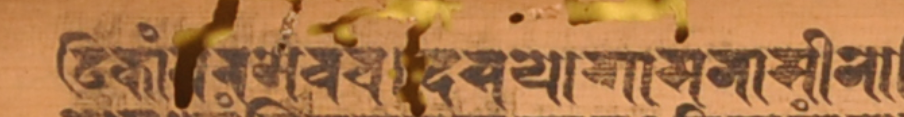
\includegraphics[scale=.3]{images/dasayoga_msNa.png}

\smallskip

\hspace{2em}[\skt{spha}]\textit{ṭikāṃ×ram} [= \skt{°kāṃbaram}] \skt{eva ca} $|$ \skt{daśayogāsanāsīno}

\medskip

\msL\ (\fol381v) gives:
\smallskip

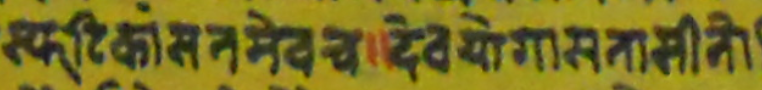
\includegraphics[scale=.3]{images/dasayoga_msL.png}
\smallskip

\hspace{2em}\skt{sphaṭikāṃsatam eva ca $||$ devayogāsanāsīto}

\smallskip
\noindent
supplying \skt{sa} for the lost syllable and misreading the 
damaged \skt{da} as \skt{de} and the \skt{śa} as \skt{va}.


\bigskip
\bigskip

Here \msNa\ (\fol39v) reads:

\smallskip
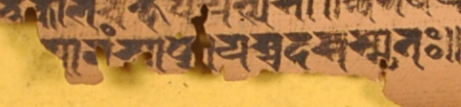
\includegraphics[scale=.5]{images/japoyoga_msNa.png}

\smallskip
[\skt{japo yogas tapo}] \skt{dhyānaṃ svādhyāyaś ca daśa smṛtaḥ} 
\smallskip

\noindent
with \textit{dhyā} and \textit{svā} damaged;

\medskip

\msL\ (\fol381r) cannot read the bit that 
is completely lost, and it misreads 
the damaged \skt{dhyānaṃ} as \skt{dhānaṃ}, \skt{svādhyā} as \skt{sādhu}:
\smallskip

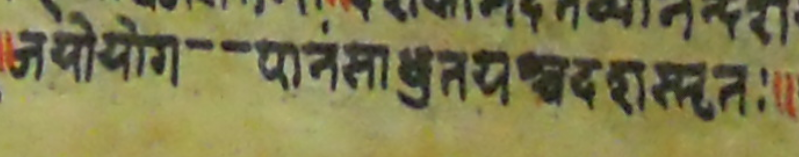
\includegraphics[scale=.3]{images/japoyoga_msL.png}

\bigskip
\bigskip

In the next example, the text is supposed to read
\skt{kare gṛhya tapodhanam $|$ tataḥ so 'ntarhitas{ }tatra tenaiva}.

\msNa\ (\fol39r) gives:
\smallskip

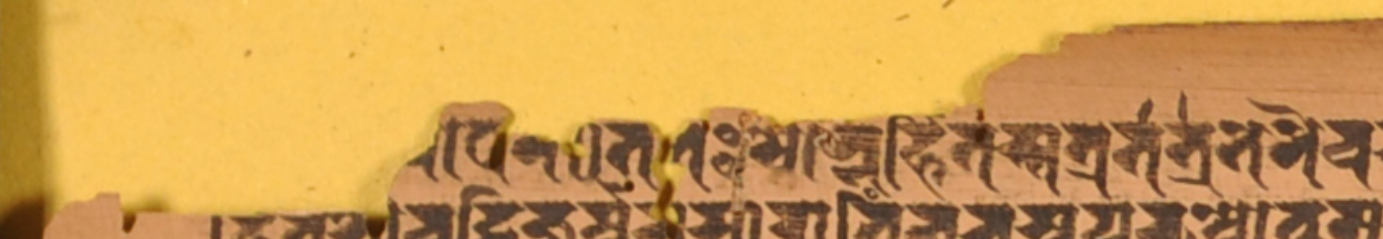
\includegraphics[scale=.21]{images/hitas_msNa.png}

\hspace{2em}[\skt{kare}] \skt{x x x x x x dha\uncl{na tataḥ so 'ntar}hitas tatra tenaiva}
\medskip

\msL\ (\fol380r) gives:
\smallskip

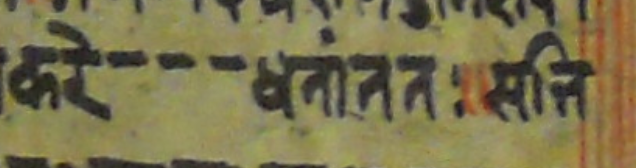
\includegraphics[scale=.3]{images/hitas01_msL.png}
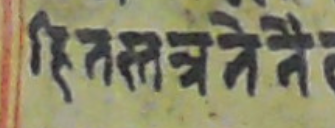
\includegraphics[scale=.3]{images/hitas02_msL.png}

\hspace{2em}\skt{kare - - - dhatāṃ tataḥ $||$ sati hitas tatra tenaiva}
\smallskip

\noindent
trying to make sense of the fragments. The examples above
suggest that \msL\ was copied directly from \msNa\
when the damage had already been done to \msNa. For this reason,
I have not collated its readings for \VSS\ chapters 1--12.


\medskip


%1) Śivadharmaśāstra, %(serial no. 634), fols.~1v--63r; 
%2) Śivadharmottara, %  (s. no. 635) fols.~64r--143v; 
%3) Śivadharmasaṃgraha, % (s. no. 633), fols.~144r--217v;
%4) Umāmaheśvarasaṃvāda, % (s. no. 652), fols.~218v-- 263v; 
%5) Śivopaniṣad, %(s. no. 636), fols.~264r--297v; 
%6) Uttarottaramahāsaṃvāda, % (s. no. 654), fols.~298r--324r;
%7) Vṛṣasārasaṃgraha, % (s. no. 657), fols.~325r--390r;
%8) Dharmaputrikā. % (s. no. 608), fols.~391r--406r.


\medskip
\subsection{Naraharinath's edition}

\mysubsubsection{(N)\Ed}{Ed}
Much has been said of Yogi Naraharinath's pioneering
but problematic edition (the \emph{editio princeps}) 
of the Śivadharma corpus
(\mycite{NaraharinathaSivadharma1998}): 
see e.g.\
\mycitep{DeSiminiGods2016}{66, n.\ 190};
\citeyear{DeSiminiLachmann2017}, 542,
\mycitep{BisschopUniversal2018}{58--59},
\mycitep{SaivaUtopia2021}{55}. My impression of the
text of the \VSS\ in Naraharinath's edition is that its quality is
considerably inferior to those of the other texts of the corpus.
It may or may not be Naraharinath's fault; others must have
been involved in the process of transcription, and the number and
nature of the innumerable mistakes all over the text may also suggest
a general problem with the typesetting process. Nevertheless
I have recorded the readings found in this publication for all 
twelve chapters given in my critical edition.

\vfill
\pagebreak


\section{Editorial policies}

\begin{quote}
- orthography: deviant orth, sandhi, punctuation?
- avagrahas usually supplied but sometimes found in the MSS, not used by me for crasis (e.g. a+a=ā)
- daṇḍas: usually 4 pādas to a verse, but I have made arbitrary decisions based on sense-units 
  because none of the sources really indicate where a verse ends (||).
- falsifications everywhere on purpose and accidentally
\end{quote}

SDh MSS from Nepal

stemma...

